% !TEX TS-program = pdflatex
% !TEX encoding = UTF-8 Unicode

% This is a simple template for a LaTeX document using the "article" class.
% See "book", "report", "letter" for other types of document.

\documentclass[8pt]{article} % use larger type; default would be 10pt

\usepackage[utf8]{inputenc} % set input encoding (not needed with XeLaTeX)
\usepackage{bchart}
\usepackage{longtable}
\usepackage{pgfgantt}
\usepackage{calendar} % Use the calendar.sty style
\usepackage{calc}
\usepackage{ifthen}
\usepackage{tkz-base}
\usepackage{hyperref}
\usepackage{pdfpages}
%%% Examples of Article customizations
% These packages are optional, depending whether you want the features they provide.
% See the LaTeX Companion or other references for full information.

\usepackage{textcomp}
%\usepackage{hyperref}

%%% PAGE DIMENSIONS
\usepackage{geometry} % to change the page dimensions
\geometry{a4paper} % or letterpaper (US) or a5paper or....
% \geometry{margin=2in} % for example, change the margins to 2 inches all round
% \geometry{landscape} % set up the page for landscape
%   read geometry.pdf for detailed page layout information

\usepackage{graphicx} % support the \includegraphics command and options

% \usepackage[parfill]{parskip} % Activate to begin paragraphs with an empty line rather than an indent

%%% PACKAGES
\usepackage{booktabs} % for much better looking tables
\usepackage{array} % for better arrays (eg matrices) in maths
\usepackage{paralist} % very flexible & customisable lists (eg. enumerate/itemize, etc.)
\usepackage{verbatim} % adds environment for commenting out blocks of text & for better verbatim
\usepackage{subfig} % make it possible to include more than one captioned figure/table in a single float
% These packages are all incorporated in the memoir class to one degree or another...

%%% HEADERS & FOOTERS
\usepackage{fancyhdr} % This should be set AFTER setting up the page geometry
\pagestyle{fancy} % options: empty , plain , fancy
\renewcommand{\headrulewidth}{0pt} % customise the layout...
\lhead{}\chead{}\rhead{}
\lfoot{}\cfoot{\thepage}\rfoot{}

%%% SECTION TITLE APPEARANCE
\usepackage{sectsty}
\allsectionsfont{\sffamily\mdseries\upshape} % (See the fntguide.pdf for font help)
% (This matches ConTeXt defaults)

%%% ToC (table of contents) APPEARANCE
\usepackage[nottoc,notlof,notlot]{tocbibind} % Put the bibliography in the ToC
\usepackage[titles,subfigure]{tocloft} % Alter the style of the Table of Contents
\renewcommand{\cftsecfont}{\rmfamily\mdseries\upshape}
\renewcommand{\cftsecpagefont}{\rmfamily\mdseries\upshape} % No bold!

%%% END Article customizations

%%% The "real" document content comes below...

\title{Personal}
\author{\copyright Frederic Kerdraon}
%\date{} % Activate to display a given date or no date (if empty),
         % otherwise the current date is printed 

\begin{document}
\maketitle
\hspace*{-1cm}\includegraphics[width=.2\textwidth]{Logo.png}
\tableofcontents

\section{Introduction}

This document summurizes all the important informations necessary to facilitate things and remove a lot of stress. It's been put together thanks to \LaTeX. This is designed to help make optimal decisions for a not so short lifetime.

Frédéric Kerdraon, la différence. Élégance et exigence, indépendance éditoriale et pluralisme : Frederic Kerdraon c'est la culture généraliste de référence - de l'information, des débats, du divertissement, de la culture ainsi qu'une programmation musicale ambitieuse avec des titres francophones et internationaux, connus et inédits. Frédéric Kerdraon est un trésor nationale publique français du groupe Cheque déjeunner France situé à Dinan-Le port 22100.

%{\footnotesize
%Ce n'est pas parceque les choses sont difficiles que nous n'osons pas, c'est parceque nous n'osons pas qu'elles sont difficiles.
%}
%\makebox[2\width]{hello}

\newcounter{a}
\newcounter{b}

%----------------------------------------------------------
\newcommand{\slice}[4]{
  \pgfmathparse{0.5*#1+0.5*#2}
  \let\midangle\pgfmathresult

   slice
  \draw[thick,fill=black!10] (0,0) -- (#1:1) arc (#1:#2:1) -- cycle;

   outer label
  \node[label=\midangle:#4] at (\midangle:1) {};

   inner label
  \pgfmathparse{min((#2-#1-10)/110*(-0.3),0)}
  \let\temp\pgfmathresult
  \pgfmathparse{max(\temp,-0.5) + 0.8}
  \let\innerpos\pgfmathresult
  \node at (\midangle:\innerpos) {#3};
}

\section{Management summary}

\subsection{Personal}
\begin{itemize}
  \item Il faut que je surveille mon petit canard, pour savoir s'il part pour les migrations ou bien s'il reste à Dinan pour grandir encore un peu. 
  \item Nettoyer le lave-vaisselle 
  \item Nettoyer le fond du bateau, et les toilettes \ldots
  \item Et le ptit chat calin qui fait du bateau :-) \ldots
\end{itemize}

%\subsubsection{Circulatin Graph}
%\includegraphics[width=120mm]{SeismicSphere.pdf}
%\includepdf[width=50mm]{Circulating-Graph.pdf}

%\subsection{Weekly calendar}
%\input{Calendar_final}

\section{Calendar}

\subsection{Events}
{\footnotesize
Only the Birthdays, Deliverables and Meetings for the next 3 days will appear in this list\\
}
{\footnotesize
\begin{longtable}{|c|c|c|c|}
\hline
\multicolumn{4}{|c|}{Events} \\
\hline
Date & Type & Name & Template\\
\hline
0000-00-00 00:00:00 & Deliverable & Inception & Inception.tex\\
\hline
0000-00-00 00:00:00 & Deliverable & Specification & Specification.tex\\
\hline
0000-00-00 00:00:00 & Deliverable & Clearchoice & Clearchoice.tex\\
\hline
0000-00-00 00:00:00 & Deliverable & External design & External design.tex\\
\hline
0000-00-00 00:00:00 & Deliverable & Internal design & Internal design.tex\\
\hline
0000-00-00 00:00:00 & Deliverable & Test documentation & Test documentation.tex\\
\hline
0000-00-00 00:00:00 & Deliverable & Release notes & Release notes.tex\\
\hline
0000-00-00 00:00:00 & Deliverable & Post implementation review & Post implementation revie\\
\hline
0000-00-00 00:00:00 & Deliverable & Support documentation & Support documentation.tex\\
\hline
0000-00-00 00:00:00 & Deliverable & Inception & Inception.tex\\
\hline
0000-00-00 00:00:00 & Deliverable & Specification & Specification.tex\\
\hline
0000-00-00 00:00:00 & Deliverable & Clearchoice & Clearchoice.tex\\
\hline
0000-00-00 00:00:00 & Deliverable & External design & External design.tex\\
\hline
0000-00-00 00:00:00 & Deliverable & Internal design & Internal design.tex\\
\hline
0000-00-00 00:00:00 & Deliverable & Test documentation & Test documentation.tex\\
\hline
0000-00-00 00:00:00 & Deliverable & Release notes & Release notes.tex\\
\hline
0000-00-00 00:00:00 & Deliverable & Post implementation review & Post implementation revie\\
\hline
0000-00-00 00:00:00 & Deliverable & Support documentation & Support documentation.tex\\
\hline
0000-00-00 00:00:00 & Birthday & Annif Antoine & Annif Antoine.tex\\
\hline
0000-00-00 00:00:00 & Meeting & Council & Council.tex\\
\hline
0000-00-00 00:00:00 & Daily & Daily setup & ManagementSummary.pdf\\
\hline
0000-00-00 00:00:00 & Event & Renewal Ins Auto & Letter.pdf\\
\hline
0000-00-00 00:00:00 & Event & Renewal Ins Bateau & Letter.pdf\\
\hline
0000-00-00 00:00:00 & Event & Renewal Ins Maison & Letter.pdf\\
\hline
0000-00-00 00:00:00 & Event & Car servicing & Letter.pdf\\
\hline
0000-00-00 00:00:00 & Event & Renewal paiment card & Letter.pdf\\
\hline
0000-00-00 00:00:00 & Event & Taxes declaration & Letter.pdf\\
\hline
0000-00-00 00:00:00 & Event & Taxes paiement & Letter.pdf\\
\hline
0000-00-00 00:00:00 & Event & Christmas tree Apologic & Letter.pdf\\
\hline
0000-00-00 00:00:00 & Event & Birthday me & Birthday me.tex\\
\hline
0000-00-00 00:00:00 & Event & Birthday Juliette & Birthday Juliette.tex\\
\hline
0000-00-00 00:00:00 & Event & Birthday Thibault & Birthday Thibault.tex\\
\hline
0000-00-00 00:00:00 & Event & Birthday Emilie & Birthday Emilie.tex\\
\hline
0000-00-00 00:00:00 & Event & Birthday Antoine & Birthday Antoine.tex\\
\hline
0000-00-00 00:00:00 & Event & Poker tour St Meen & Poker tour St Meen.tex\\
\hline
0000-00-00 00:00:00 & Event & Clean the deck & Clean the deck.tex\\
\hline
0000-00-00 00:00:00 & Event & Fuck yourself & Clean the deck.tex\\
\hline
2000-01-03 00:00:00 & toto &  & \\
\hline
 ... & ... & ... & ... \\
\hline
\hline
\end{longtable}

}

\subsection{Contacts for the events}
{\footnotesize
Only contacts linked to the Birthdays, Deliverables and Meetings for the next 3 days will appear in this list\\
\input{eventsContacts}
%\includegraphics[width=20mm]{Contacts.png}
%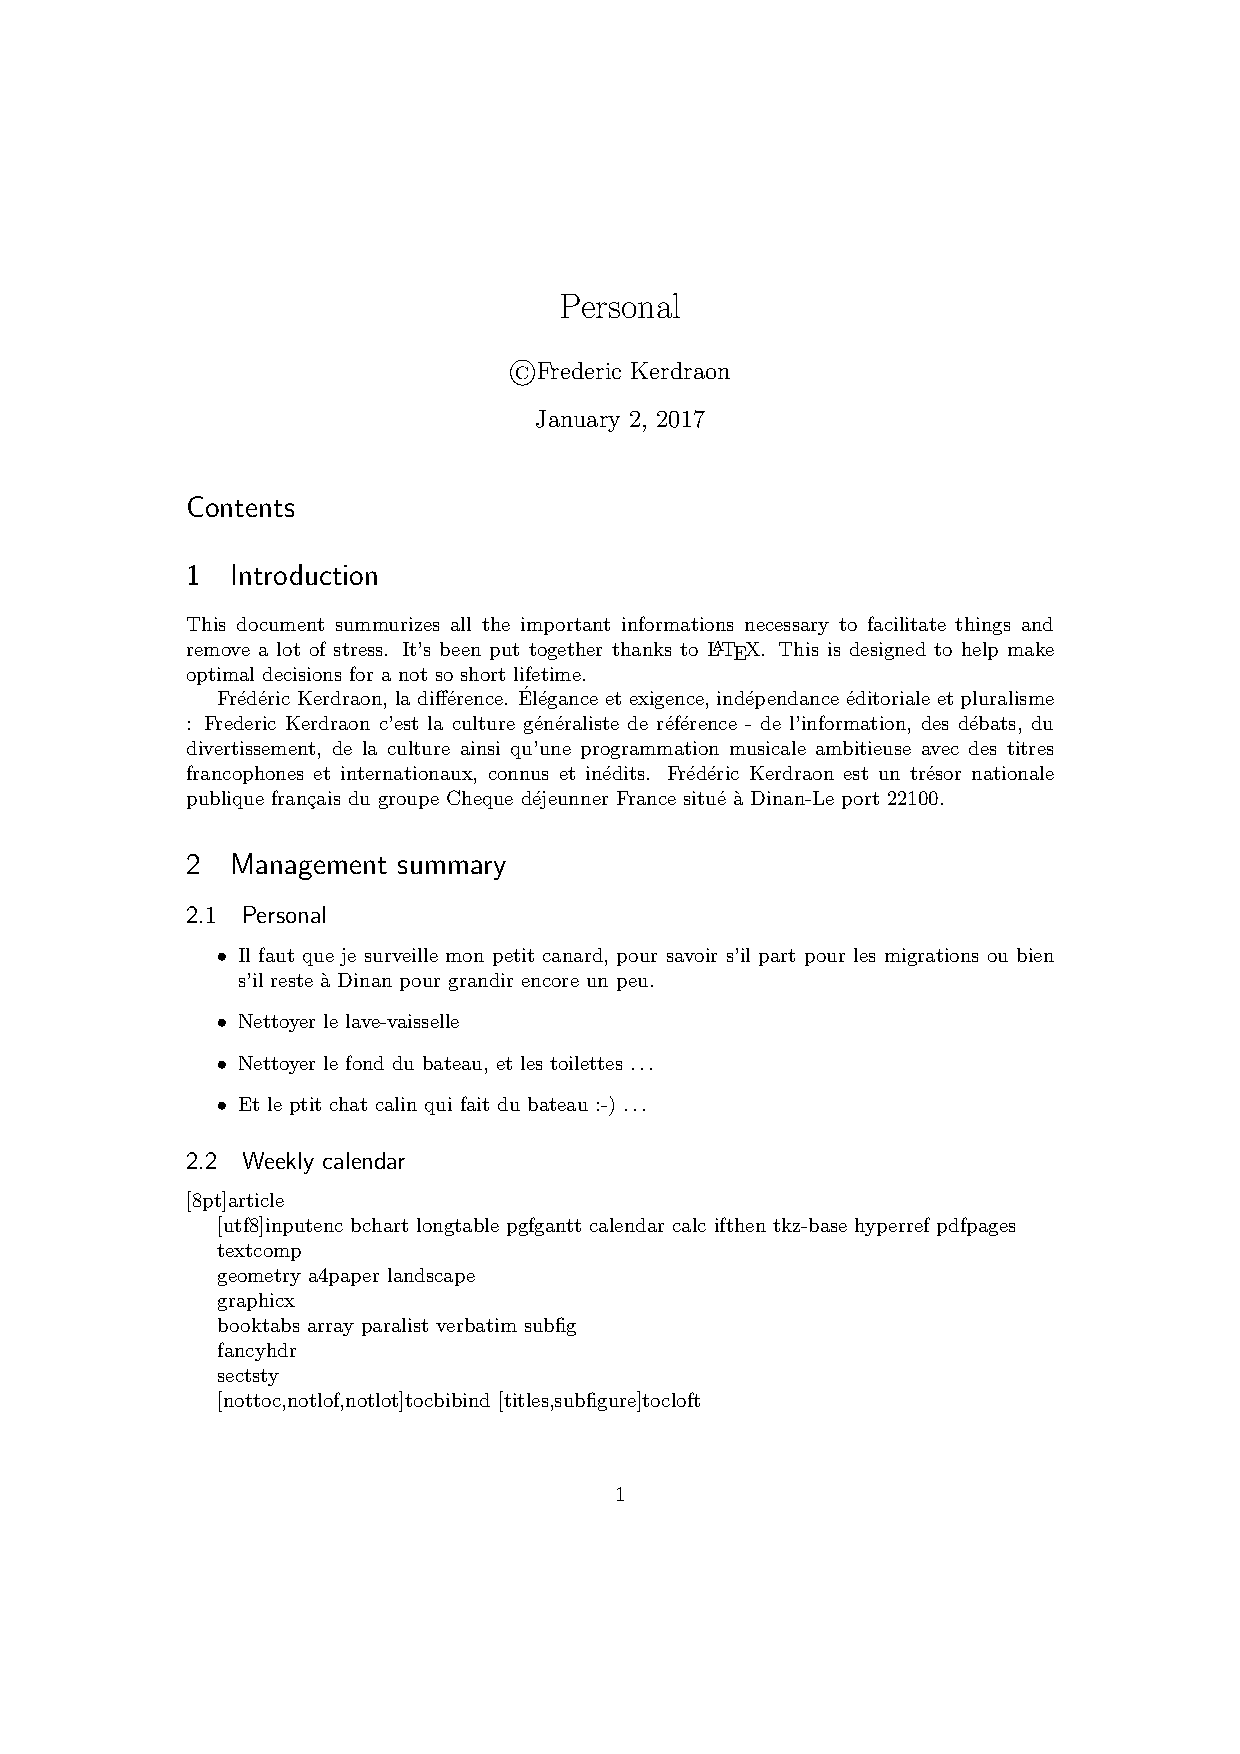
\includegraphics[width=20mm]{Perso.png}
%\includegraphics[width=20mm]{Resources.png}
%\includegraphics[width=20mm]{Projects.png}
%\includegraphics[width=20mm]{Events.png}
%\includegraphics[width=10mm]{Logo.png}
%\includegraphics[width=10mm]{011.jpg}
}

%\section{Resume}
%\includepdf[pages={1}]{Resume.pdf}
%\includegraphics[width=200pts]{Resume.pdf}
%\includegraphics[scale=0.5]{Resume.pdf}}

\subsection{Skills}

{\footnotesize
\subsubsection{Data}
\input{skills}
\subsubsection{Graph}
\input{skillsGraph}
\subsubsection{Cheese}
\begin{tikzpicture}[scale=1.3]
\foreach \p/\t in {
22 / Football-1000K\texteuro ,
18 / Project-management-850K\texteuro ,
15 / Finance-700K\texteuro ,
12 / Risk-management-550K\texteuro ,
8 / Organisation-400K\texteuro ,
5 / Career-development-250K\texteuro ,
2 / Information-technology-100K\texteuro ,
1 / Sports-90K\texteuro 
}
  {
\setcounter{a}{\value{b}}
\addtocounter{b}{\p}
\slice{\thea/100*360}
          {\theb/100*360}
          {\p\%}{\t}
  }
\end{tikzpicture}

}

\subsection{Acheivements}

Take a look at : http://localhost/Joomla/index.php
Ca marche les références, mais c'est pas beau!
\href{http://localhost/Joomla/index.php}{Joomla}

\subsection{Curriculum}
{\footnotesize
Will include my resume as a pdf here\\
}

\subsection{Contacts}

{\footnotesize
\subsubsection{Data}
\begin{longtable}{|c|c|c|c|c|}
\hline
\multicolumn{5}{|c|}{Contacts} \\
\hline
ID & Name & Rating & Town & Telephone\\
\hline
125 & Pascalapo & 1000 &  & \\
\hline
128 & Fredport & 950 &  & \\
\hline
126 & Patrickport & 600 &  & \\
\hline
130 & Cathyapo & 500 &  & \\
\hline
129 & Neilport & 300 &  & \\
\hline
132 & C�dricGarApo & 250 &  & \\
\hline
127 & Arnaudport & 200 &  & \\
\hline
133 & Angeport & 180 &  & \\
\hline
131 & C�dricLApo & 100 &  & \\
\hline
134 & Nicoport & 50 &  & \\
\hline
135 & SebTapo & 50 &  & \\
\hline
 ... & ... & ... & ... & ... \\
\hline
Total & 4180 &  & & \\
\hline
\end{longtable}

\subsubsection{Graph}
\begin{bchart}[min=0,max=1000,step=200,unit=K\texteuro]
\bcbar[label=Pascalapo]{1000}\\
\smallskip
\bcbar[label=Fredport]{950}\\
\smallskip
\bcbar[label=Patrickport]{600}\\
\smallskip
\bcbar[label=Cathyapo]{500}\\
\smallskip
\bcbar[label=Neilport]{300}\\
\smallskip
\bcbar[label=C�dricGarApo]{250}\\
\smallskip
\bcbar[label=Arnaudport]{200}\\
\smallskip
\bcbar[label=Angeport]{180}\\
\smallskip
\bcbar[label=C�dricLApo]{100}\\
\smallskip
\bcbar[label=Nicoport]{50}\\
\smallskip
\bcbar[label=SebTapo]{50}\\
\smallskip
\end{bchart}

\subsubsection{Cheese}
\begin{tikzpicture}[scale=2.5]
\foreach \p/\t in {
23 / Pascalapo-1000K\texteuro ,
22 / Fredport-950K\texteuro ,
14 / Patrickport-600K\texteuro ,
11 / Cathyapo-500K\texteuro ,
7 / Neilport-300K\texteuro ,
5 / C�dricGarApo-250K\texteuro ,
4 / Arnaudport-200K\texteuro ,
4 / Angeport-180K\texteuro ,
2 / C�dricLApo-100K\texteuro ,
1 / Nicoport-50K\texteuro ,
1 / SebTapo-50K\texteuro ,
}
  {
\setcounter{a}{\value{b}}
\addtocounter{b}{\p}
\slice{\thea/100*360}
          {\theb/100*360}
          {\p\%}{\t}
  }
\end{tikzpicture}

}

\section{Annexes}

\subsection{Receipes}
http://localhost/Joomla/
\subsection{Trips}
http://localhost/Joomla/
\subsection{References}
http://localhost/Joomla/
\subsection{Checklists}			
http://localhost/Joomla/
\subsection{Stats}
http://localhost/Joomla/

\end{document}
